\chapter{序論}
\label{chap:intro}

本章では,本研究の研究背景と研究目的について説明する.
\secref{sec:background}で研究背景,
\secref{sec:purpose}で研究目的,
\secref{sec:structure}で本論文の構成について述べる.

\section{研究背景}\label{sec:background}
\indent
音楽演奏を題材としたアニメーションは多く存在する.
テレビで放映されたアニメーションの例を挙げると,『のだめカンタービレ』,『けいおん!』,『響け!ユーフォニアム』が相当する.
これらのアニメーションは,セル画であったり3DCGであったり,製作方法がさまざまであるが,いずれも実際に演奏する演奏者の身体の動きに近い演奏シーンが生成されている.
楽器の輝きや形状なども忠実に再現されている.\\
\indent
一方,楽器を演奏するキャラクタの運指や身体の動きに注目すると,音楽と動きが完全に同期されていないことがあり,違和感を感じる.
特に速いフレーズや,複雑なリズムを演奏するシーンで,このようなアーティファクトが起きやすい.
また,表情からも不自然さを感じることがある.
実際にアンケートをとったところ,吹奏楽やオーケストラの経験の有無に関わらず,不自然だと感じると回答した者が半数以上であった.\figref{fig:q1}は,その集計結果である.
\begin{figure}[h]
	\centering
	\subcaptionbox{\textgt{吹奏楽・オーケストラ経験者の回答}
		\label{fig:ans1_1}}{
		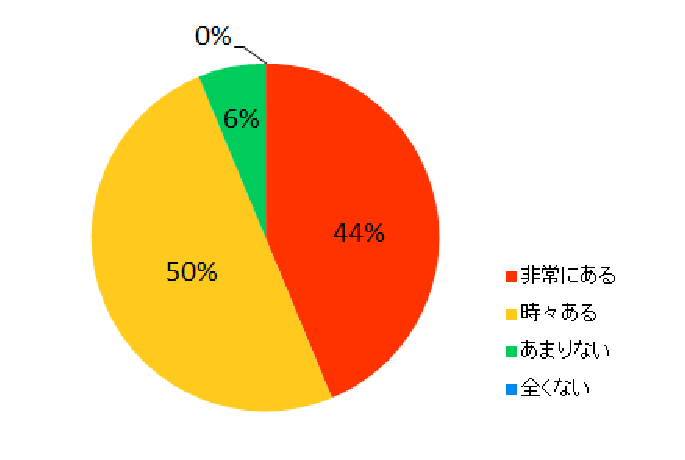
\includegraphics[width=7cm]{fig/chap1/Q1-1.eps}}
	\subcaptionbox{\textgt{吹奏楽・オーケストラ未経験者の回答}
		\label{fig:ans1_2}}{
		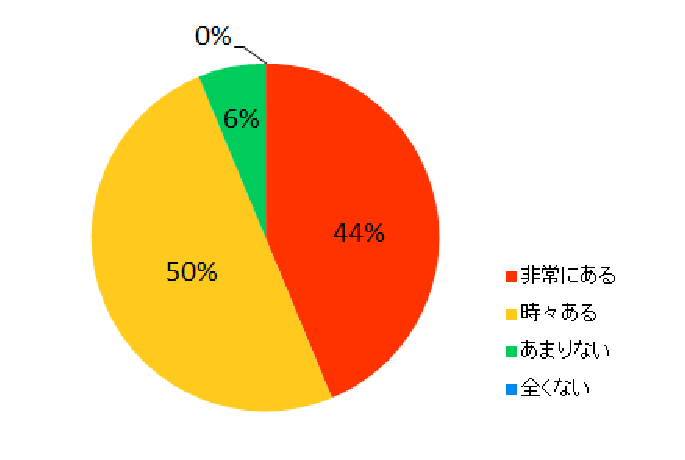
\includegraphics[width=7cm]{fig/chap1/Q1-2.eps}}
	\caption{演奏アニメーションが不自然であると感じることがあるかどうか}
	\label{fig:q1}
\end{figure}

しかし,すべての音と身体の動きや表情を合わせるには,多くの時間と労力が必要となる.

\section{研究目的}\label{sec:purpose}
\indent
\secref{sec:background}節で述べた課題を解消するため,本研究では,管楽器を演奏するキャラクタの吹奏アニメーションを,音源から自動的に生成することを目指す.
より具体的には,実際の演奏アニメーション制作フローに沿わせるため,楽曲は楽器(ウインドシンセサイザ)を用いて,MIDI(Musical Instrument Digital Interface)音源として生成する.
次に,作成した楽曲を解析することにより,吹奏の情報を得る.
最後に,得られた情報をキャラクタの身体の動きや表情,そして管楽器に適用することにより,音源に同期した自然な吹奏アニメーションを実現する.
提案手法の対象ユーザはアニメータとし,最終的にはアニメータのアニメーション制作時間と労力の削減を目的とする.
また,本研究は,同研究室学士4年の武内と共同で行った.
武内が担当した部分については,その旨を明記する.

\section{本論文の構成}\label{sec:structure}
本論文は次章以降,以下のように構成される.\\
\indent
次章では関連研究を説明する.
第3章では提案手法の仕組みを説明する.
そして,第4章では自動生成結果を述べ,この結果に対する評価をまとめる.
最後に第5章で結論を述べ,今後の課題に言及する.\\
\indent
なお,本研究の成果はVisual Computing/グラフィクスとCAD合同シンポジウム2017にてポスター発表\cite{vc}を行った.そして,映像表現・芸術科学フォーラム2018(2018年3月),Cyberworlds(2018年8月)において発表を行う予定である.